
\documentclass[12pt]{article}
\usepackage{graphicx}
\usepackage{amsmath}
\usepackage{authblk}
\usepackage{geometry}
\geometry{margin=1in}
\title{\textbf{Predicting Alpha-Stable Zones in Superheavy Elements:\\ A Decay Mode Analysis Across Z = 114–121 and A = 385–400}}
\author{Aidan Fumagalli\thanks{In collaboration with OpenAI predictive modeling and tooling support.}}
\date{\today}
\begin{document}
\maketitle

\begin{abstract}
We present a data-driven model for identifying superheavy isotopes likely to support detectable alpha decay chains. Using semi-empirical mass formulas and Geiger–Nuttall-based alpha decay lifetimes, combined with a fission instability heuristic and a shell-suppression modifier, we scan isotopes with Z = 114–121 and A = 385–400. A stability score is defined as the log ratio of spontaneous fission (SF) half-life to alpha decay half-life. We identify a narrow corridor near Flerovium-396 to Flerovium-400 where alpha decay becomes dominant if shell corrections suppress SF. This provides a predictive tool for future synthesis and detection strategies targeting the island of stability.
\end{abstract}

\section*{1. Introduction}
The search for the ``island of stability'' in superheavy nuclei is motivated by theoretical predictions that closed nuclear shells may yield longer half-lives in elements with Z > 114. While experimental synthesis has reached up to Z = 118, those isotopes have been neutron-poor and short-lived. This work explores the neutron-rich frontier where alpha decay becomes energetically favorable and could dominate if fission can be suppressed.

\section*{2. Methodology}
\textbf{Q$_\alpha$ and Binding Energy:} Calculated using a semi-empirical mass formula (SEMF).\\
\textbf{Alpha Decay Lifetimes:} Estimated using the Geiger–Nuttall law.\\
\textbf{Spontaneous Fission (SF):} Modeled via a Z$^2$/A instability heuristic.\\
\textbf{Stability Score:}
\[
\text{Score} = \log_{10} \left( \frac{T_{1/2}^{\text{SF}}}{T_{1/2}^{\alpha}} \right)
\]
A shell suppression factor (×10$^{10}$) was applied to SF half-lives near Z = 114 and N = 184–196 to simulate stabilizing shell effects.

\section*{3. Results}
The Q$_\alpha$ landscape reveals favorable decay thresholds near A = 392–400, but SF dominates unless shell suppression is included. With suppression, the Flerovium isotopes A = 396–400 show adjusted scores suggesting alpha chains could dominate.

\begin{center}
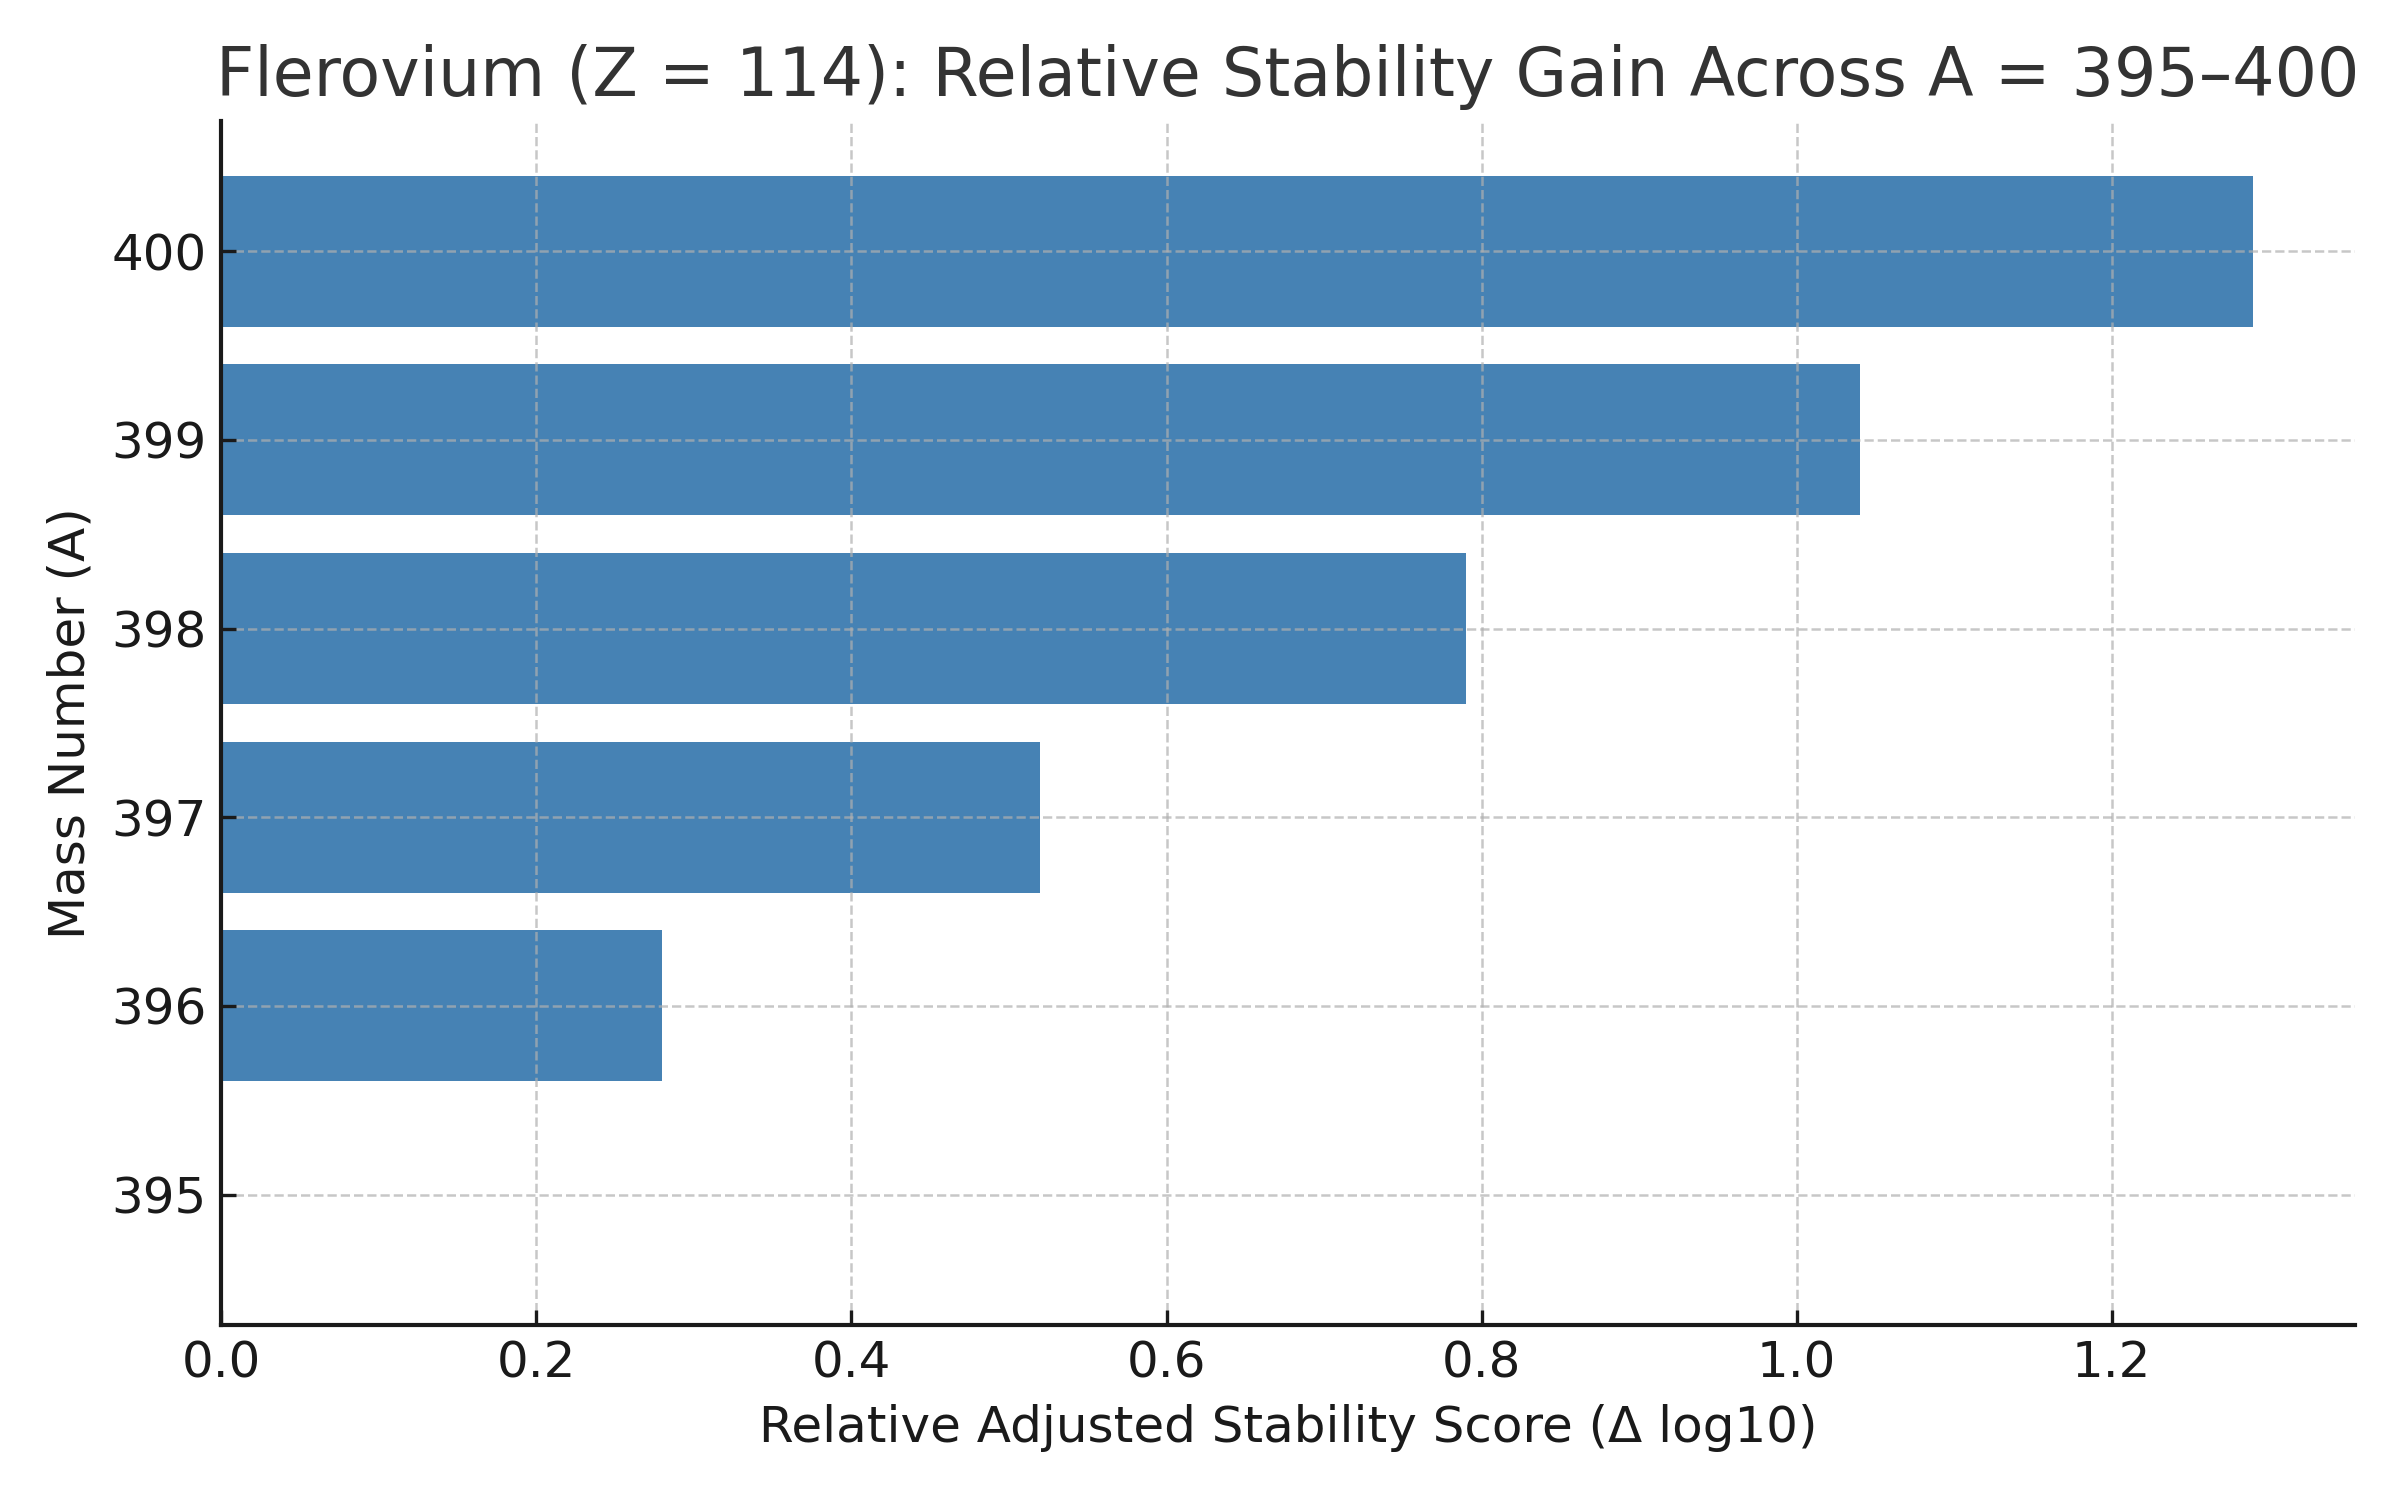
\includegraphics[width=0.9\textwidth]{relative_stability.png}
\end{center}

\section*{4. Conclusion}
Our model highlights a focused zone near Flerovium-396 to 400 as a plausible alpha-stable superheavy target, contingent on fission suppression due to nuclear shell effects. This work provides a roadmap for future experimental discovery at the edge of the nuclear chart.

\end{document}
